\documentclass[10pt,letter]{article}
\usepackage{amsmath}
\usepackage{setspace}
\onehalfspacing
\usepackage{amssymb}
\usepackage{graphicx}
\usepackage{hyperref}

\usepackage{fullpage}

\newcommand{\rhintbox}[1]{\begin{center} \singlespacing
  \framebox[.9\textwidth][c]{\begin{minipage}{.8\textwidth}#1
\end{minipage}}\end{center}\onehalfspacing}

\newcommand{\R}{R}

\newcommand{\bi}{\begin{itemize}}
\newcommand{\ei}{\end{itemize}}

\begin{document}

\title{Bias/Variance Tradeoff Notes}

\author{Professor Adam Glynn}

\date{September 30, 2019}

\maketitle 
\noindent

\subsection*{Sampling Distribution of the Sample Mean}
\begin{itemize}
\item $Y_i \sim_{iid}$ with $E[Y_i]=\mu$ and $V[Y_i]=\sigma^2$.
\item Describe as a sampling problem and draw table and distribution
\item Derive $E[\bar{Y}]$, what does this mean in terms of bias?
\item Derive $V[\bar{Y}]$, how does this relate to $V[Y_i]$?
\item Draw sampling distribution on top of distribution of an observation.
\end{itemize}

\subsection*{Sampling Distribution of the Sample Standard Deviation}
\begin{itemize}
\item Put $S^2 = \frac{1}{n-1}\sum_{i=1}^n (Y_i-\bar{Y})^2$ on the board and ask what it is
\item Derive $E[S^2]$, 
\begin{align*}
(n-1)\cdot S^2 &= \sum_{i=1}^n (Y_i-\bar{Y})^2 \\
&= \sum_{i=1}^n Y_i^2 -  2\sum_{i=1}^n Y_i\cdot \bar{Y} +  \sum_{i=1}^n \bar{Y}^2\\
&= \sum_{i=1}^n Y_i^2 - 2 \bar{Y} \sum_{i=1}^n Y_i  +  \sum_{i=1}^n \bar{Y}^2\\
&= \sum_{i=1}^n Y_i^2 - 2 \bar{Y} n \bar{Y}  +  n \bar{Y}^2\\
&= \sum_{i=1}^n Y_i^2 -   n \bar{Y}^2\\
\end{align*}
\begin{align*}
E[(n-1)\cdot S^2] &= (n-1)E[(n-1) S^2] \\
&= \sum_{i=1}^n E[Y_i^2] -   n E[\bar{Y}^2]\\
&= n E[Y_i^2] -   n E[\bar{Y}^2]\\
\end{align*}
\begin{align*}
E[Y_i^2] &= V[Y_i] + E[Y_i]^2\\
&= \sigma^2 + \mu^2 \\ 
E[\bar{Y}^2] &= \sigma^2/n + \mu^2 \\
E[Y_i^2]  - E[\bar{Y}^2] &= \sigma^2 - \sigma^2/n \\
&= \frac{n-1}{n} \sigma^2
\end{align*}

\item what does this mean in terms of bias? Draw sampling distribution.

\end{itemize}

\subsection*{Sampling Distribution with $\frac{1}{n}$}

\begin{itemize}
\item Put $\tilde{S}^2 = \frac{1}{n}\sum_{i=1}^n (Y_i-\bar{Y})^2$ on the board.
\item Derive $E[\tilde{S}^2]$, 

\begin{align*}
E[\tilde{S}^2] &= E[\frac{n-1}{n}S^2] \\
&= \frac{n-1}{n} E[S^2] \\
&= \frac{n-1}{n} \sigma^2
\end{align*}
\item what does this mean in terms of bias?
\item write the $V[\tilde{S}^2]$ in terms of $V[S^2]$
\begin{align*}
V[\tilde{S}^2] &= V[\frac{n-1}{n}S^2] \\
&=  \left( \frac{n-1}{n}\right)^2 V[S^2] 
\end{align*}
\item draw sampling distribution for $\tilde{S}^2$ on top of sampling distribution for $S^2$.
\item discuss bias/variance tradeoff implicit in the comparison
\item discuss $MSE = Bias^2 + Var$
\end{itemize}

\subsection*{Regression}

\begin{verbatim}
# Population
N <- 10000
x <- rnorm(N,mean=4,sd=1)
y <- -2*x + .5*x^2 + rnorm(N)

plot(x,y,xlim=c(0,8),ylim=c(-5,15),main="Population")
lines(seq(0,8,.1),-2*seq(0,8,.1) + .5*seq(0,8,.1)^2, col="red")
abline(v=4,col="red")
abline(lm(y~x),col="green")

# f(4) = 0
-2*4 + .5*4^2
\end{verbatim}


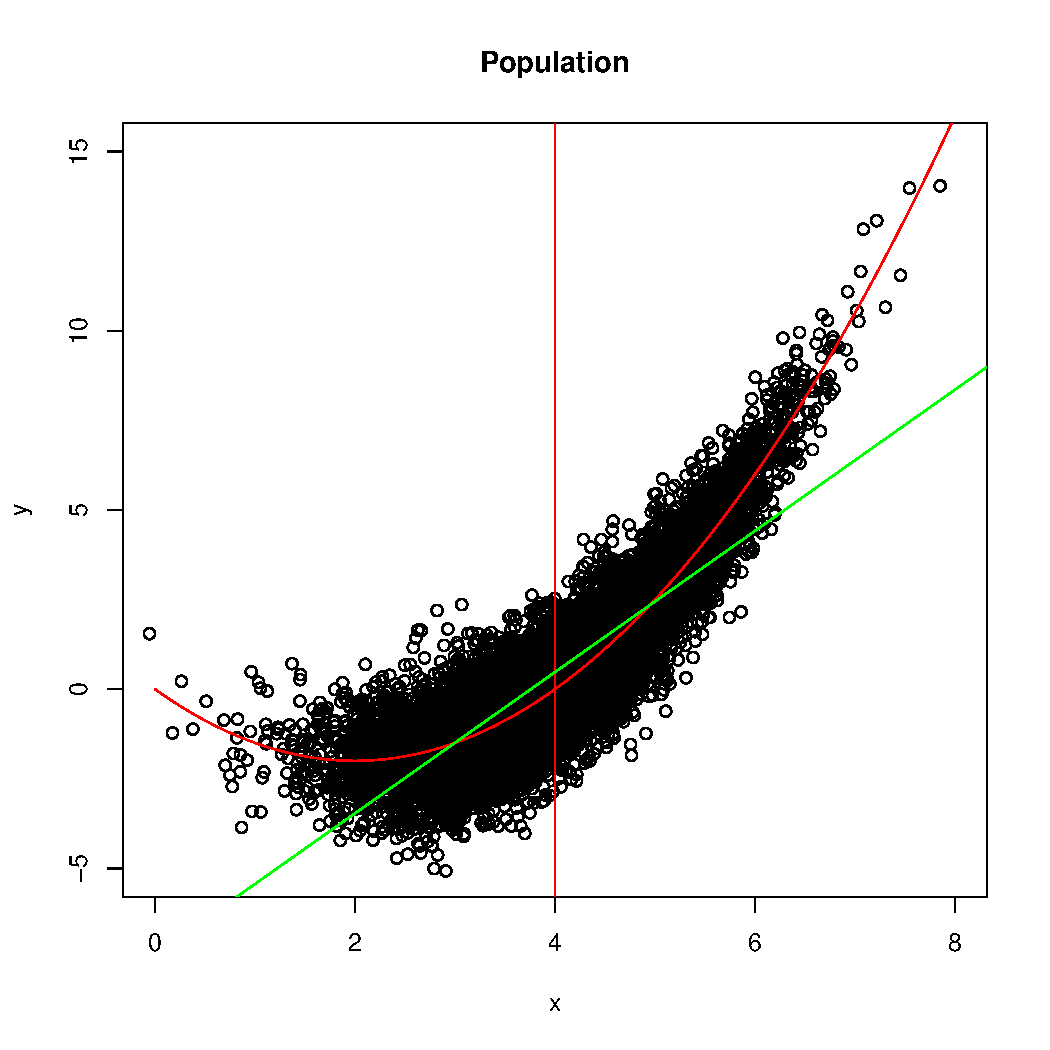
\includegraphics[scale=.7]{Population}

\newpage

\begin{verbatim}
# Observed Data
set.seed(123)
n <- 3
i <- sample(1:N,size=n,replace = TRUE)
plot(x[i],y[i],xlim=c(0,8),ylim=c(-5,15))
abline(v=4,col="red")
abline(lm(y[i]~x[i]),col="green")
quad <- lm(y[i]~x[i]+I(x[i]^2))
lines(seq(0,8,.1),quad$coef[1] + quad$coef[2]*seq(0,8,.1) + quad$coef[3]*seq(0,8,.1)^2, col="red")
\end{verbatim}

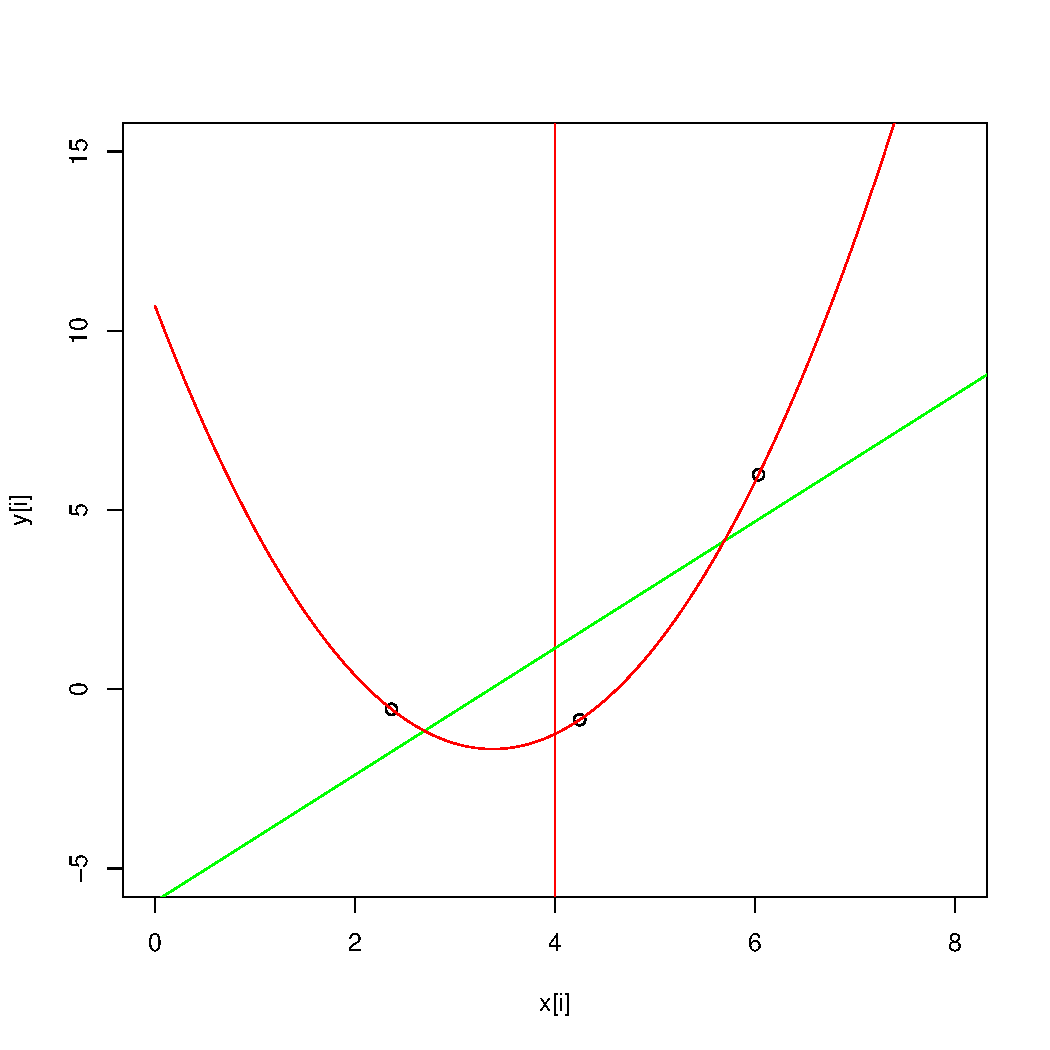
\includegraphics[scale=.7]{Sample}


\newpage

\begin{verbatim}
# Sampling Distributions
S <- 10000
fhat.lin <- rep(0,S)
fhat.quad <- rep(0,S)
n <- 3
for(s in 1:S){
	i <- sample(1:N,size=3,replace = TRUE)
	lin <- lm(y[i]~x[i])
	fhat.lin[s] <- lin$coef[1] + lin$coef[2]*4
	quad <- lm(y[i]~x[i]+I(x[i]^2))
	fhat.quad[s] <- quad$coef[1] + quad$coef[2]*4 + quad$coef[3]*(4^2)	
}
plot(density(fhat.lin[fhat.lin > -10 & fhat.lin < 10]),col="green",main="Sampling Distributions")
lines(density(fhat.quad[fhat.quad > -10 & fhat.quad < 10 & !is.na(fhat.quad)]),col="red")
abline(v=0,col="red")
\end{verbatim}

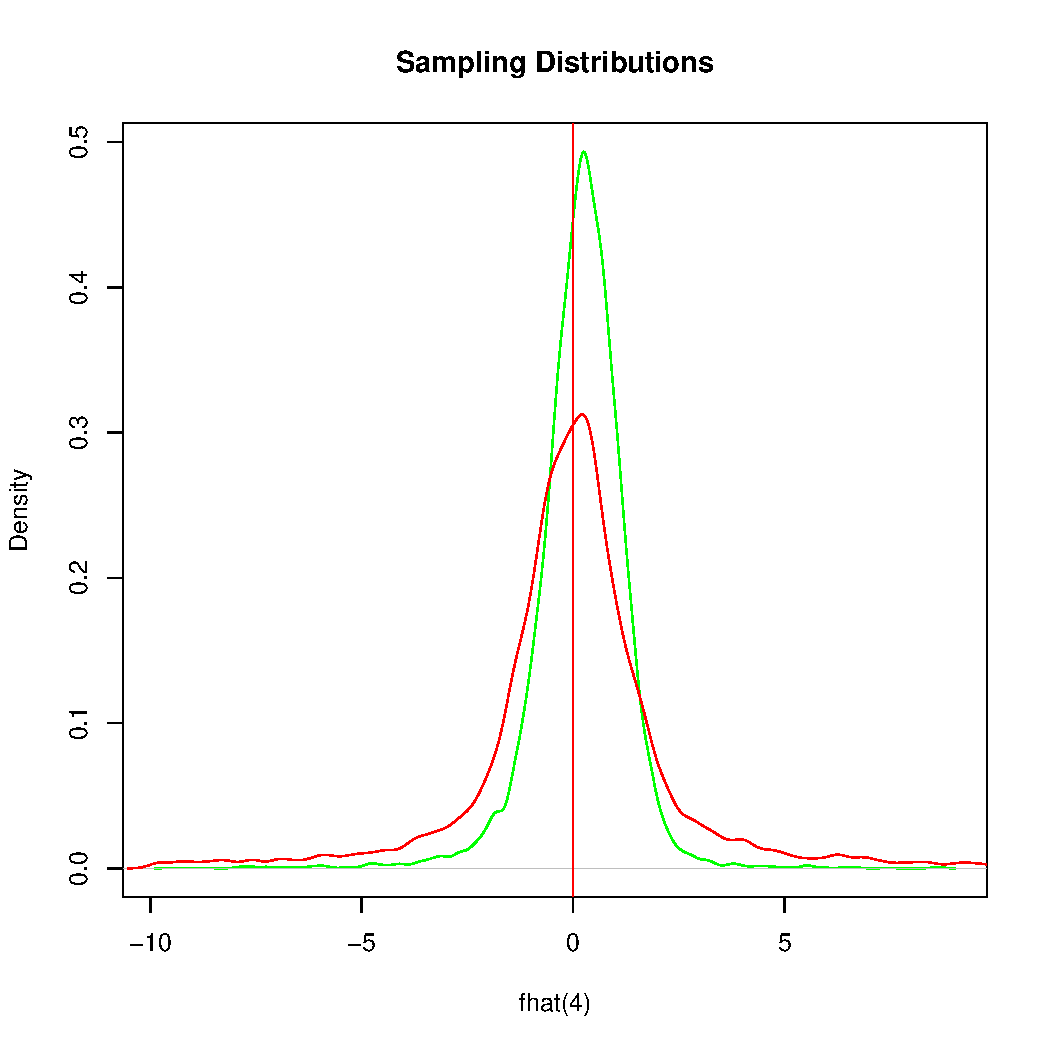
\includegraphics[scale=.7]{SamplingDistributions}

\newpage

\begin{verbatim}
> #Bias
> mean(fhat.lin[fhat.lin > -10 & fhat.lin < 10])
[1] 0.1908053
> mean(fhat.quad[fhat.quad > -10 & fhat.quad < 10],na.rm=TRUE)
[1] 0.004055125

> #Var
> var(fhat.lin[fhat.lin > -10 & fhat.lin < 10])
[1] 1.191539
> var(fhat.quad[fhat.quad > -10 & fhat.quad < 10],na.rm=TRUE)
[1] 5.279145
\end{verbatim}


\end{document}

